\documentclass[conference]{IEEEtran}
\IEEEoverridecommandlockouts

\usepackage{cite}
\usepackage{amsmath,amssymb,amsfonts}
\usepackage{algorithmic}
\usepackage{graphicx}
\usepackage{hyperref}
\usepackage[nameinlink, capitalise]{cleveref}
\usepackage{float}
\usepackage{textcomp}
\usepackage{xcolor}
\def\BibTeX{{\rm B\kern-.05em{\sc i\kern-.025em b}\kern-.08em
    T\kern-.1667em\lower.7ex\hbox{E}\kern-.125emX}}
    
% -----------------------------
% -----    HYPER SETUP    -----
% ----------------------------- 

\hypersetup {
    colorlinks = true, 
    linkcolor = blue, 
    citecolor = blue, 
    urlcolor = blue, 
}

% -------------------------
% -----    SPACING    -----
% -------------------------

% Sets vertical spacing for tables
\renewcommand{\arraystretch}{1.1}

% Defines equation spacing
\makeatletter
\g@addto@macro\normalsize{%
  \setlength\abovedisplayskip{20pt}
  \setlength\belowdisplayskip{20pt}
  \setlength\abovedisplayshortskip{10pt}
  \setlength\belowdisplayshortskip{20pt}
}
\makeatother
    
\begin{document}

\graphicspath{ {./assets/} }

\title{Evaluating Global Delta Correlation (G/DC) Prefetcher on Simulated Hardware}

\author{\IEEEauthorblockN{Håkon Harnes} \and \IEEEauthorblockN{Vetle Harnes}}

\maketitle

% --------
% ABSTRACT 
% --------

\begin{abstract}
The advancements in processor performance in recent years by far exceeds the improvements in memory access latency. Numerous techniques have been developed to compensate for this, among others prefetching. This paper presents a prefetching algorithm called Global Delta Correlation (G/DC). G/DC is a correlation based distance prefetcher that uses a Global History Buffer (GHB) to keep track of memory accesses and an Index Table (IT) for faster look-ups into the GHB. The M5 hardware simulator was used to simulate the prefetcher implementation. The SPEC CPU2000 benchmark suite was used to evaluate its performance against other prefetchers. The paper also compares the three different implementations of the G/DC scheme, which is width, depth and hybrid. We found the G/DC prefetcher was able to achieve an average speedup of 5\%. 
\end{abstract}

% ------------
% INTRODUCTION
% ------------

\section{INTRODUCTION}
\iffalse 
The introduction section introduces the larger research area the paper is a part of and illustrates the concrete problem(s) at hand the paper tries to solve. It explains the proposed solution from a 20.000 feet abstraction level. Furthermore, it states the contributions of the paper and briefly highlights its main results. It finishes with an outline of the paper, giving a short explanation of the contribution/meaning of each section.
\fi

In the last half-century microprocessor and semiconductor technology has faced a rapid development in an effort to match the ever growing dependence on technology. This has allowed us to put exponentially more transistors into integrated circuits to significantly increase the clock frequency of microprocessors \cite{b3}. This yielded an on average growth in clock frequency of 40\% between 1988 and 2002, and even though it is currently stagnating it has increased by 2\% yearly \cite{b11}. On the other hand, the improvement in main memory bandwidth and latency has been lagging behind. This is what is referred to as the "Memory wall" \cite{b4}. This indicates that the main performance bottleneck in modern computers is memory access latency, not the theoretical amount of Instructions Per Cycle (IPC) the processor can execute.

\begin{figure}[h]
    \centering
     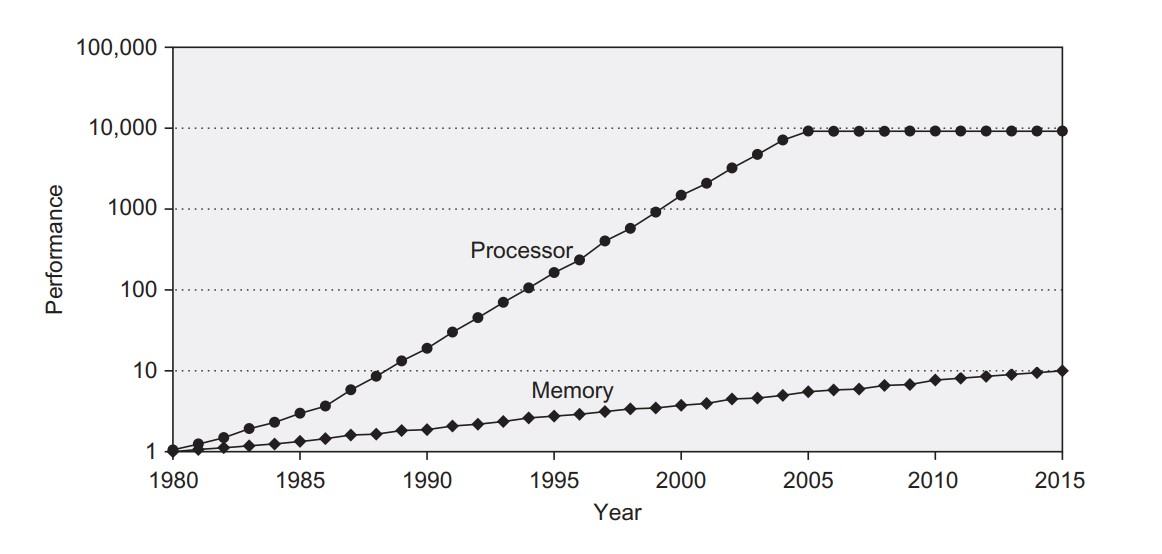
\includegraphics[width=9cm]{assets/processor-memory-gap.jpg}
    \vspace{-6mm}
    \caption{The memory wall represents the increasing gap between processor and memory performance \cite{b4}.}
    \label{fig:mirror}
\end{figure}

To compensate for this bottleneck multiple levels of high performance caches were introduced. These caches took advantage of the principles of spatial and temporal locality. The idea was to store the required data in smaller and faster memory devices closer to the processor \cite{b7}. Although it was a good solution, limited cache sizes and associativity led to the eviction of useful data. This introduced the need for predicting what data accesses would be required in the future, and then fetch them in advance. This is referred to as prefetching. Prefetching exploits memory access patterns to decrease the memory bottleneck. 

This paper evaluates the performance of the Global Delta Correlation (G/DC) prefetcher. G/DC is a distance prefetcher that uses delta-correlation to predict future memory accesses. It stores a list of global miss addresses in a Global History Buffer (GHB). The GHB is stored as a linked list and be accessed through an indirect indexed hash table for faster look-ups. 

The prefetcher has been simulated using a modified M5 hardware simulator \cite{m5doc} and evaluated using the SPEC CPU2000 benchmark suite \cite{b8}. The G/DC prefetcher was able to achieve a 5\% average speedup. On single tests, it was able to achieve speedups of up to 37\%. In addition, it requires little hardware overhead to implement. 

% ------------
% BACKGROUND
% ------------

\section{BACKGROUND}
\iffalse 
The background section covers knowledge that is necessary for understanding the proposed solution, but you cannot expect the audience of the paper to be familiar with. This is commonly the case when you propose solutions that incorporate knowledge from different research areas. An example would be an implementation of a compression scheme between memory and processor in order to decrease memory bandwidth utilization. It is very likely that you would need to explain the compression scheme, since most computer architecture researchers would not be familiar with 
\fi 

Cache prefetching is an efficient way to decrease the memory access latency. When implementing a cache prefetcher, it is important that the performance gain outweighs the silicone overhead. If not, it would be more beneficial to add more cores \cite{b12}.

Simple prefetchers like adjacent and strided prefetchers are based on spatial locality. The adjacent prefetcher fetches the next block in addition to the one the processor needs. The strided prefetcher is a bit more advanced. It detects memory access patterns and fetches blocks with a constant stride between them \cite{b6}.  However, these prefetchers are unable to detect more complex memory access patterns. More sophisticated prefetchers take complex correlations between memory accesses into account. To manage this added complexity, a Global History Buffer (GHB) with an Index Table (IT) can be used. 

\subsection{Global History Buffer (GHB)}
In 2004 Nesbit and Smith \cite{b1} proposed using a GHB for prefetching. The GHB is a circular First In First Out (FIFO) table, that holds the addresses of the most recent cache misses. The entries in the table stores a link pointer, which makes the GHB entries a linked list, and a global miss address. The addresses with equal indices is stored in a time-ordered sequence. This allows correlation based prefetching algorithms to perform, while needing considerably less memory. Increasing the size of the GHB allows it to store more entries, but comes at the price of using more silicone area on the chip. The GHB is depicted in \cref{fig:GHB}. 

\begin{figure}[H]
    \centering
     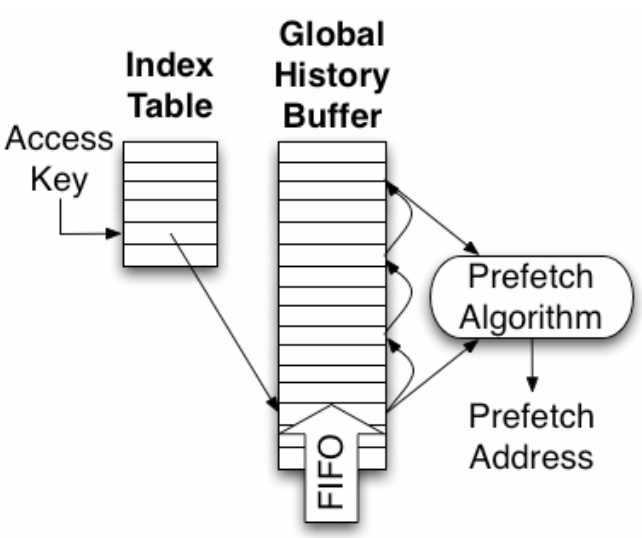
\includegraphics[width=6cm]{assets/GHB-prefetch-structure.png}
    \vspace{-2mm}
    \caption{Global History Buffer that is indexed by an index table. The data in the GHB is used as input to the prefetch algorithm \cite{b1}.}
    \label{fig:GHB}
\end{figure}

\subsection{Index Table (IT)}
The Index Table (IT) is used to access the GHB, as seen in \cref{fig:GHB}. The IT stores a list of key-pointer pairs. The pointers in the IT point to the previous GHB entry associated with the same key. This decreases the overhead of accessing the GHB substantially.

\subsection{Markov prefetching}
The Markov Prefetching is a correlation based prefetcher. Correlation based prefetching associates the given prefetched address with a correlation table that is based on earlier memory accesses \cite{b10}. If the address does not exist in the table, it is added to it. For instance, with a miss address of A, and a correlation table as depicted in \cref{fig:GHB}, Markov prefetching would prefetch the data in C and B. 

\begin{figure}[H]
    \centering
     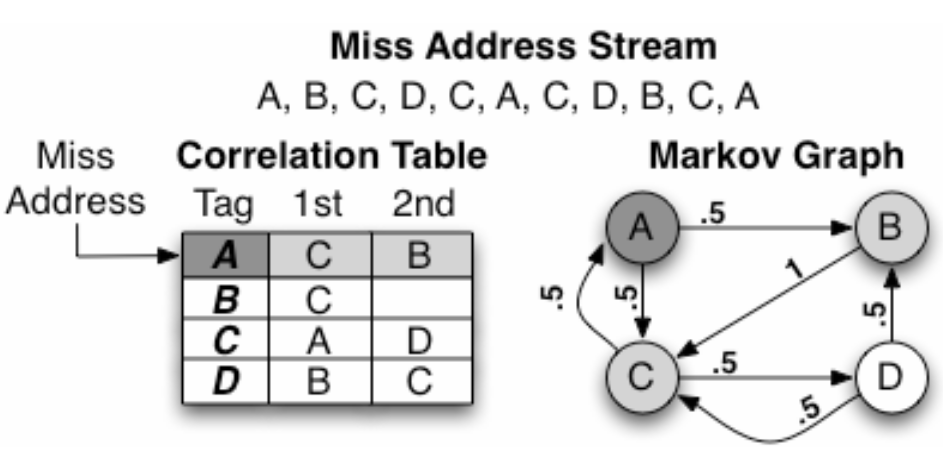
\includegraphics[width=62mm]{assets/markov-prefetch.png}
    \vspace{-2mm}
    \caption{Markov prefetching \cite{b1}.}
    \label{fig:Markov}
\end{figure}

\subsection{Distance prefetching}
Distance prefetching tries to detect many of the patterns the Markov Prefetching can accommodate while taking advantage of the strided behavior in execution \cite{b2}. Distance prefetching keeps track of the difference between successive addresses to make predictions. This allows it to reuse memory access patterns for different miss addresses. This improves on Markov's high memory requirement. When combined with the GHB one can achieve even lower memory requirements without loosing the ability to recognize dynamic memory access patterns.

\begin{figure}[H]
    \vspace{5mm}
    \centering
     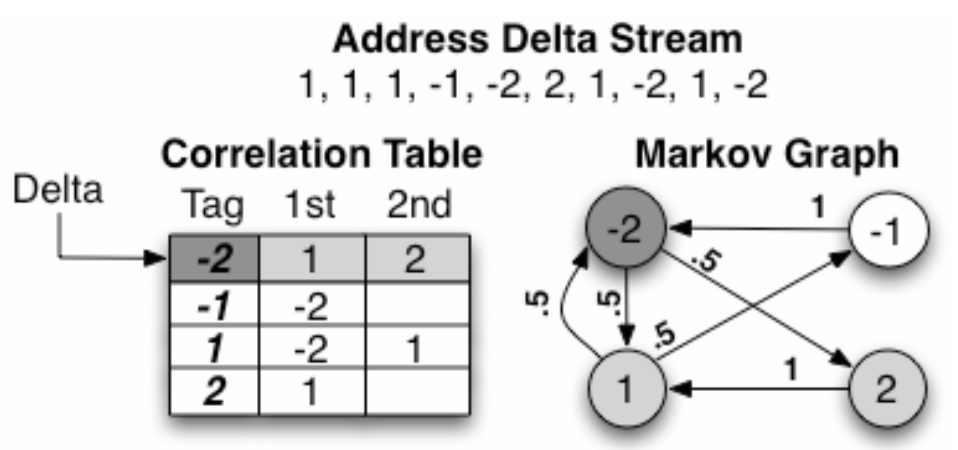
\includegraphics[width=62mm]{assets/distance-prefetching.png}
    \vspace{-2mm}
    \caption{Distance prefetching \cite{b1}.}
    \label{fig:Distance}
\end{figure}

% ------------
% THE SCHEME 
% ------------

\section{Global Delta Correlation (D/DC)}
\iffalse
This section explains your proposed solution in full detail. It needs to strike a fine balance between unnecessary implementation details and a level of abstraction that is too high. The goal is to give enough detail such that the audience of your paper is able to re-implement your scheme, but not more. Informative figures and examples are a very powerful tool for conveying necessary information to your audience, and are often worth more than a thousand words.
\fi
As proposed by Nesbit and Smith \cite{b1}, our implementation uses GHB indexed by an IT in combination with a distance based prefetcher.
The GHB address list and coordinates is maintained by a simple state machine. The GHB is implemented as a circular buffer in a FIFO manner. This means that data elements are inserted into the bottom of the list and removed from the top. This gives priority to the history with the most recent and common occurrence. When a cache miss occurs, the address is inserted into the GHB at the head pointer, and the link entry is given the current value in the index table. Then, the IT link entry is updated with a pointer to the head pointer. This process is illustrated in \cref{fig:GDC}.

The IT uses the delta as an access key to get the correct entry in the GHB. Once the correct index is obtained we check the delta stream adjacent to the delta key or similar delta keys to find the addresses we wish to prefetch. This can be seen in \cref{fig:GDC}. Here we use a delta of -2 to predict the future addresses needed. In this example we end up checking all the matching deltas (dark gray) and fetch the adjacent deltas that is later in the delta stream (light gray). We then use this to find our predicted address and prefetch it.

If the IT does not contain a pointer to a corresponding GHB entry, the prefetcher will act as a sequential prefetcher. This allows the prefetcher to keep fetching potentially useful data, even if there is no useful history present.

\begin{figure}[H]
    \centering
    \vspace{-2mm}
     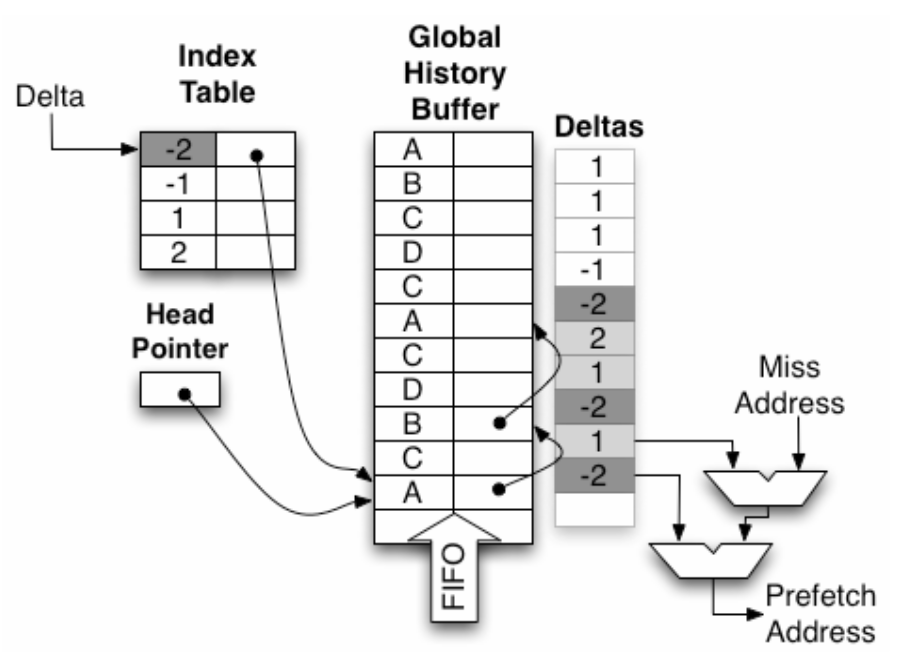
\includegraphics[width=7cm]{assets/gdc.png}
    \vspace{-2mm}
    \caption{Global Delta Correlation (G/DC) \cite{b1}.}
    \label{fig:GDC}
\end{figure}

In this paper we have implemented three variants of the G/DC prefetcher: Width, depth and hybrid. 

\subsection{Width}
Width limits the number of previous entries that are visited. For instance, with a a width of two, the prefetcher will look at the history of the two previous entries in the GHB with the same delta value. This is reflected in \cref{fig:GDC} by the curved arrows. This favours recent behaviour when deciding prefetch candidates. 

\subsection{Depth}
Depth limits the number of adjacent deltas that are visited. This is reflected in \cref{fig:GDC} by the gray shaded deltas. This enables the prefetcher to run further ahead of the actual address stream \cite{address_stream}. 

\subsection{Hybrid}
The hybrid approach combines both width and depth.

% ------------
% METHODOLOGY 
% ------------

\section{METHODOLOGY}
\subsection{Simulator}
The simulator is a modified version of the M5 hardware simulator. It is an open-source simulator based on the architecture of the DEC Alpha Tsunami system, specifically the Alpha 21264 microprocessor. It is a four-issue superscalar, out-of-order processor that can rearrange a large number of instructions, and perform speculative execution \cite{alph21264}. The specifications of the simulator used is presented in \cref{tab:m5spec}. 

The modified version of the M5 simulator presents a simplified interface to the second level (L2) cache. The interface contains methods for prefetching data, as well as information about cache accesses \cite{m5doc}. 

\begin{table}[H]
    \centering
    \begin{tabular}{l | r l}
        Specification        & Size &                   \\
        \hline
        L1 data cache        & 64   & \hspace{-4mm} KiB \\
        L1 instruction cache & 32   & \hspace{-4mm} KiB \\
        L1 cache block size  & 32   & \hspace{-4mm} KiB \\
        L2 cache size        & 1    & \hspace{-4mm} MiB \\
        L2 cache block size  & 32   & \hspace{-4mm} KiB \\
        Memory bus clock     & 400  & \hspace{-4mm} MHz \\
        Memory bus latency   & 30   & \hspace{-4mm} ns  \\
        Memory bus width     & 8    & \hspace{-4mm}     \\
    \end{tabular}
    \vspace{5mm}
    \caption{M5 simulator specifications}
    \label{tab:m5spec}
    \vspace{-5mm}
\end{table}

\subsection{Benchmark suite}
The SPEC CPU2000 benchmark suite has been used to evaluate the performance of the prefetcher. The benchmark suite contains a wide range of tests that are based on real-word user applications. They are compute-intensive applications that measure the performance of the processor, memory and compiler \cite{b8}. The benchmark suite is presented in \cref{tab:benchmarks}. 

The tests in the benchmark suite often do some initialization and setup on startup. The prefetcher evaluation is therefore performed after the tests have run for some time. The number of warm up instructions used in this paper was one billion ($10^9$) instructions. 

\begin{table}[H]
    \centering
    \begin{tabular}{l | p{4cm} }
        Benchmark & Description                    \\
        \hline
        ammp      & Computational chemistry        \\
        applu     & Partial differential equations \\
        apsi      & Weather prediction             \\
        art       & Neural network simulation      \\
        bzip2     & Compression                    \\
        galgel    & Fluid dynamics                 \\
        swim      & Shallow water modeling         \\
        twolf     & Place and route simulator      \\
        wupwise   & Quantum chromodynamics         \\
    \end{tabular}
    \vspace{5mm}
    \caption{SPEC CPU2000 benchmark suite}
    \label{tab:benchmarks}
    \vspace{-5mm}
\end{table}

\subsection{Statistics}

The statistics is used to evaluate the prefetcher performance. The terminology used in the statistics is presented in \cref{tab:terminology}. 

\begin{table}[H]
    \centering
    \begin{tabular}{l | p{4cm} }
        Term                & Description                    \\
        \hline
        IPC                 & Instructions per cycle        \\
        Cache miss          & Number of L2 cache misses      \\
        Good prefetch       & The prefetched block is referenced by the application before it is replaced. \\
        Bad prefetch        & The prefetched block is replaced without being referenced             \\
    \end{tabular}
    \vspace{5mm}
    \caption{Terminology}
    \label{tab:terminology}
    \vspace{-5mm}
\end{table}

The speedup is is a commonly used proxy for overall performance. It measures the relative performance gain. 
\[
    \text{Speedup} = \frac{\text{IPC}_{\text{With prefetcher}\phantom{ou}}}{\text{IPC}_\text{Without prefetcher}}
\]
The accuracy measures the number of useful prefetches issued by the prefetcher.
\[
    \text{Accuracy} = \frac{\text{Good prefetches}}{\text{Total prefetches}}
\]
The coverage measures how many potential candidates for prefetches that were actually identified by the prefetcher. 
\[
    \text{Coverage} = \frac{\text{Good prefetches}}{\text{Cache misses without prefetching}}
\]
The harmonic mean is a kind of average used to aggregate each benchmark speedup score into an average speedup. 
\[
    \text{Harmonic mean} = \frac{n}{\frac{1}{x_1} + \frac{1}{x_2}+\dots+\frac{1}{x_n}} = \frac{n}{\Sigma_{i=1}^n \frac{1}{x_i}}
\]

% ------------
% RESULTS
% ------------

\pagebreak 
\section{RESULTS}

\iffalse
This section presents the results of your experiments, comparing your solution to other schemes. The metrics of interest are highly dependent on the topic of research, but should optimally cover all interesting aspects of your scheme. Informative graphs or tables are the key to a good result section.

Furthermore, you need to discuss your results. You should give explanations of distinctive points and outliers in your results. It is also necessary to state why your scheme is better/worse compared to the other schemes. Thus, this section consists of two parts: the results of your experiments, as well as an explanation as to why the results are as they are.
\fi

In this section, the width, depth and hybrid variants of the G/DC prefetcher are evaluated and compared against other prefetching schemes. First, the test results are presented. The prefetcher was tested using a prefetching degree of 4, and a GHB and IT size of 256. Second, the parameter testing results are described. The prefetch degree, GHB and IT size have been tested and evaluated. 

\subsection{Test performance}

The G/DC hybrid prefetcher achieved an average speedup of 5\%, as can be seen in \cref{fig:comparison}. All three variants of G/DC outperformed the simple prefetchers, like the sequential on access, sequential on miss and tagged schemes. The hybrid variant was even able to perform on-par with DCPT. However, both DCPT-P and RPT were able to achieve higher speedups than the all of the G/DC variants. This may be caused by the fact that DCPT-P and RPT are suited for recognizing strided memory access patterns \cite{dcpt}, while G/DC is not. 

\begin{figure}[H]
    \centering
     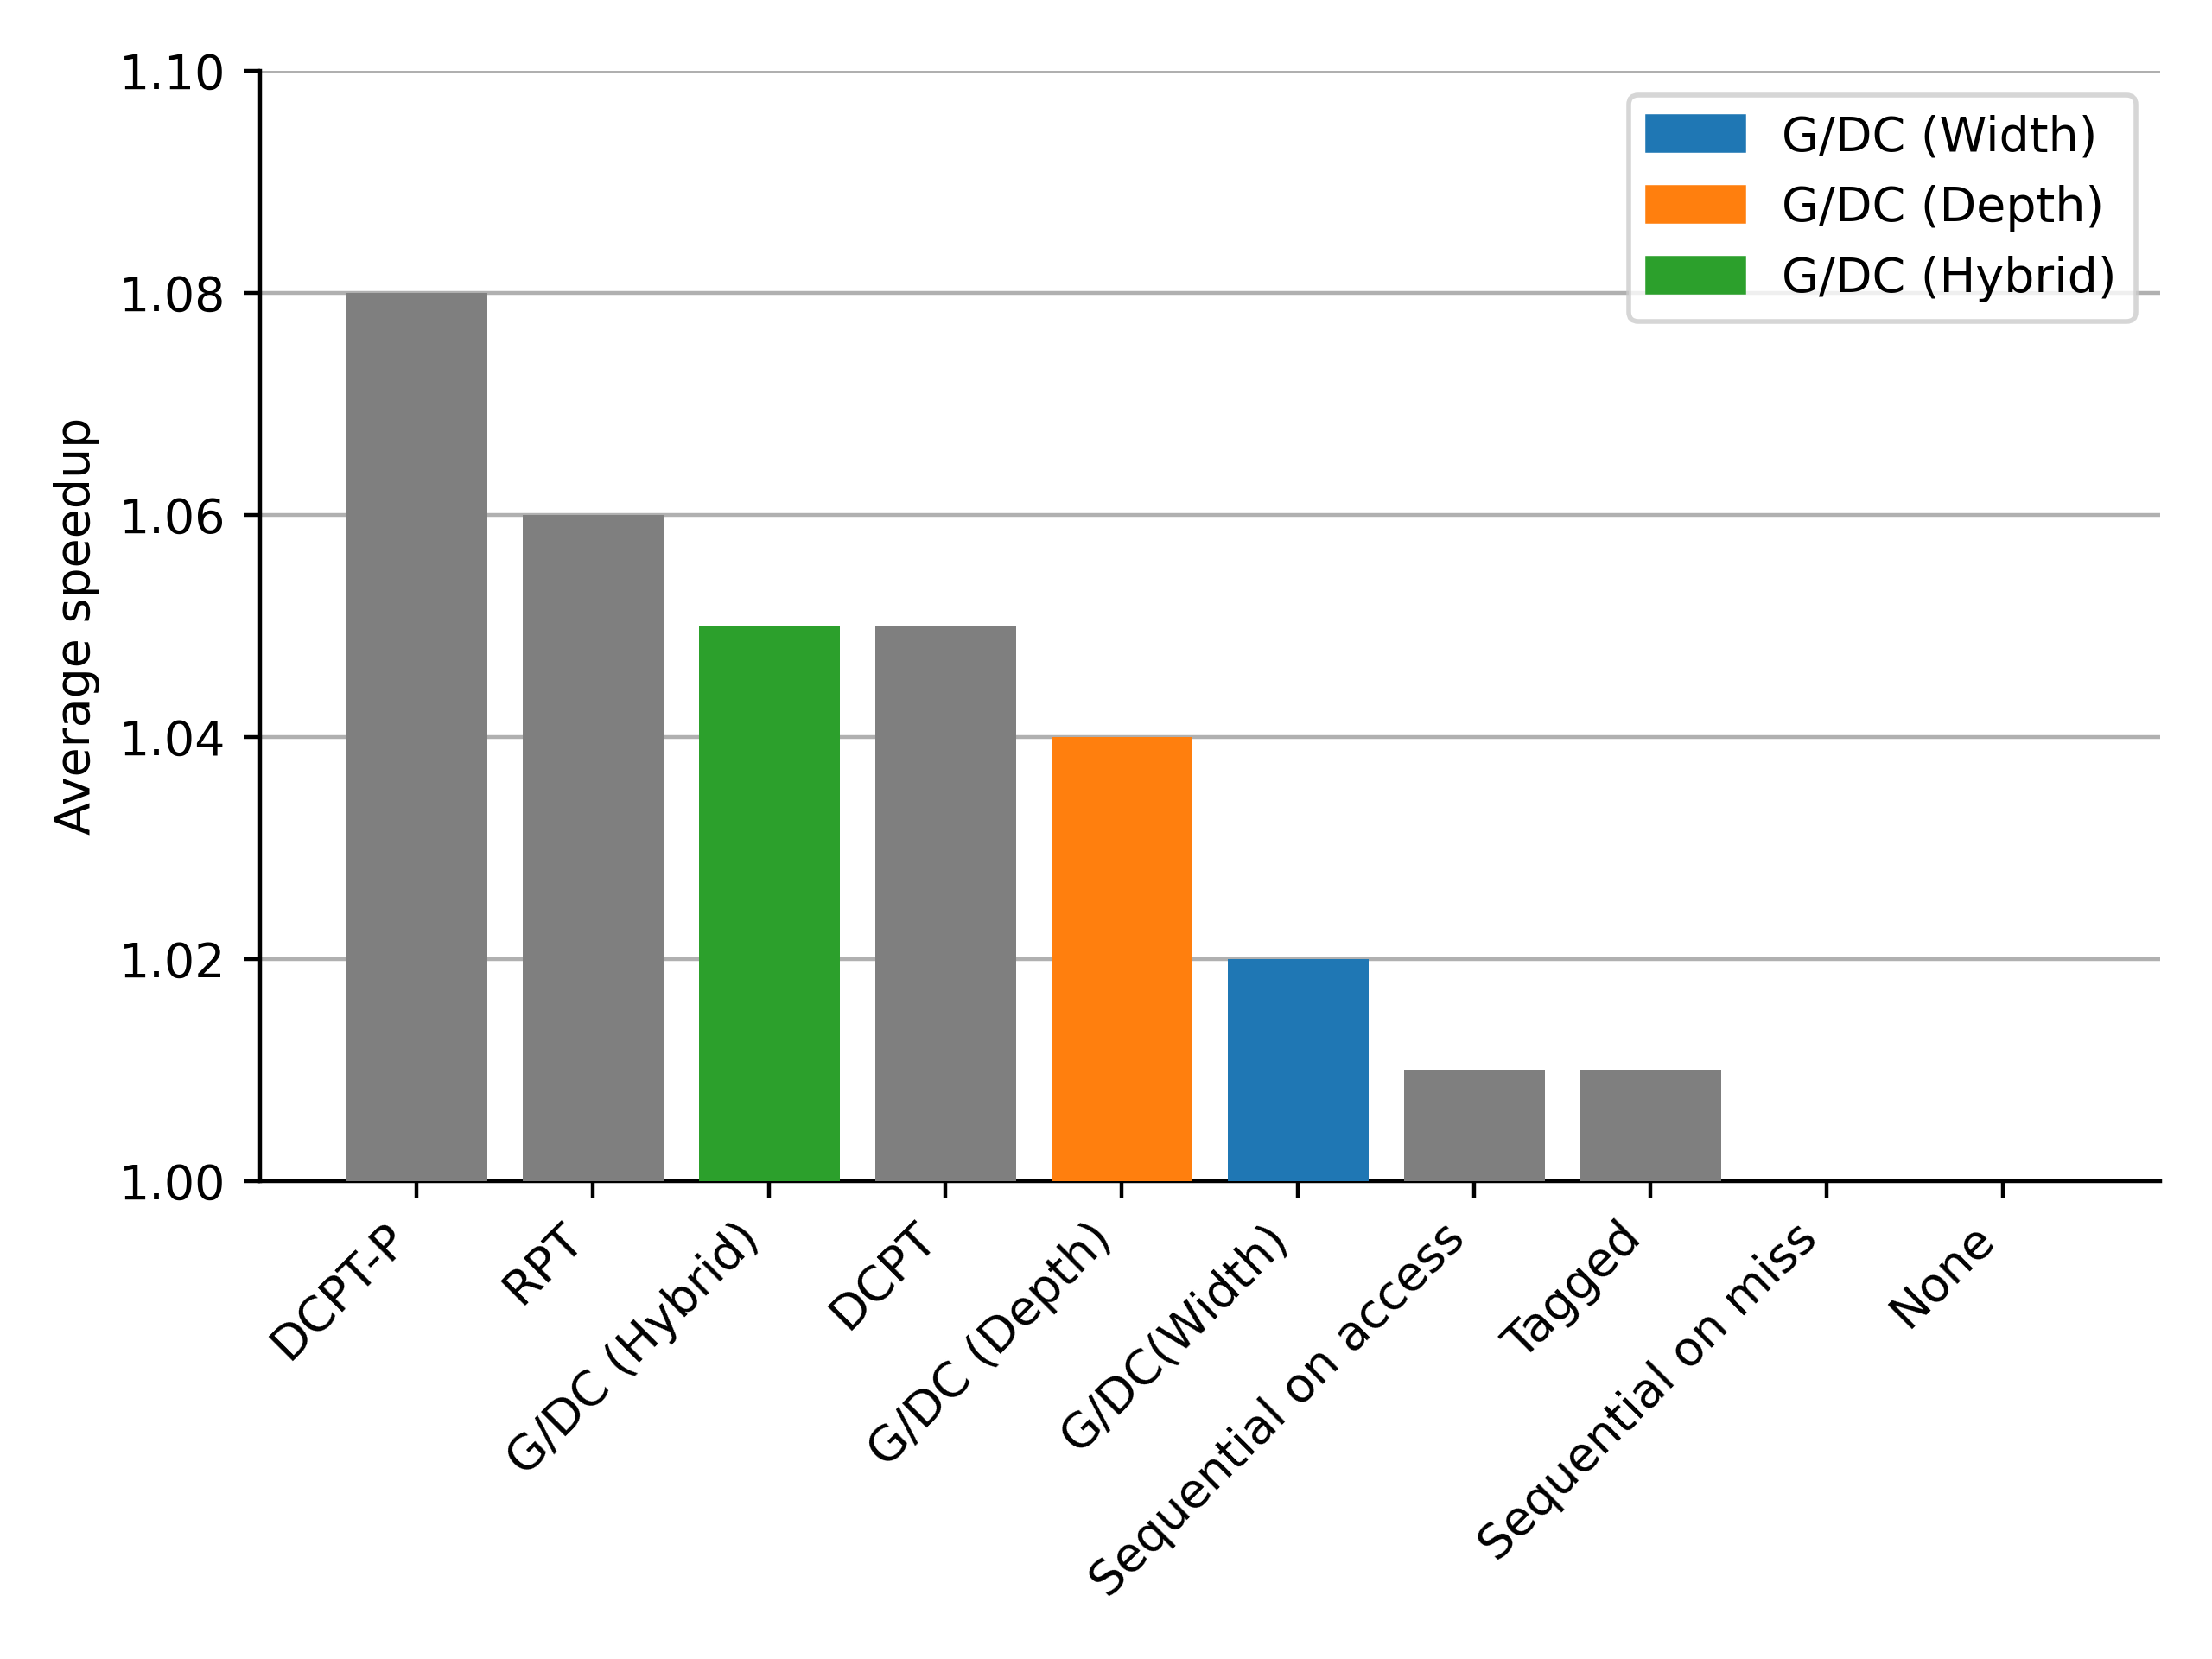
\includegraphics[width=90mm]{assets/comparison.png}
    \vspace{-7mm}
    \caption{Average speedups for the different prefetcher algorithms. }
    \label{fig:comparison}
    \vspace{-2mm}
\end{figure}

As illustrated in \cref{fig:tests}, the three G/DC variants performs similarly on the majority of the tests. The two big outliers are the ammp and swim tests. In the ammp test, the hybrid variant vastly outperformed the the others with a speedup of 37\%, followed by the depth variant at 27\%, and the width variant at 0\%. On the other hand, in the swim test, the order was reversed. This can be attributed to the hybrid prefetcher being able to access more delta-correlations before it turns into a sequential prefetcher. We could also theorize that the depth variant is more likely to have an available node with enough history to satisfy the degree than the width variant. This is likely due to the FIFO nature of the GHB, causing older entries to be evicted. This indicates that the ammp test has a higher degree of delta-correlation in it than swim does.

\begin{figure}[H]
    \centering
     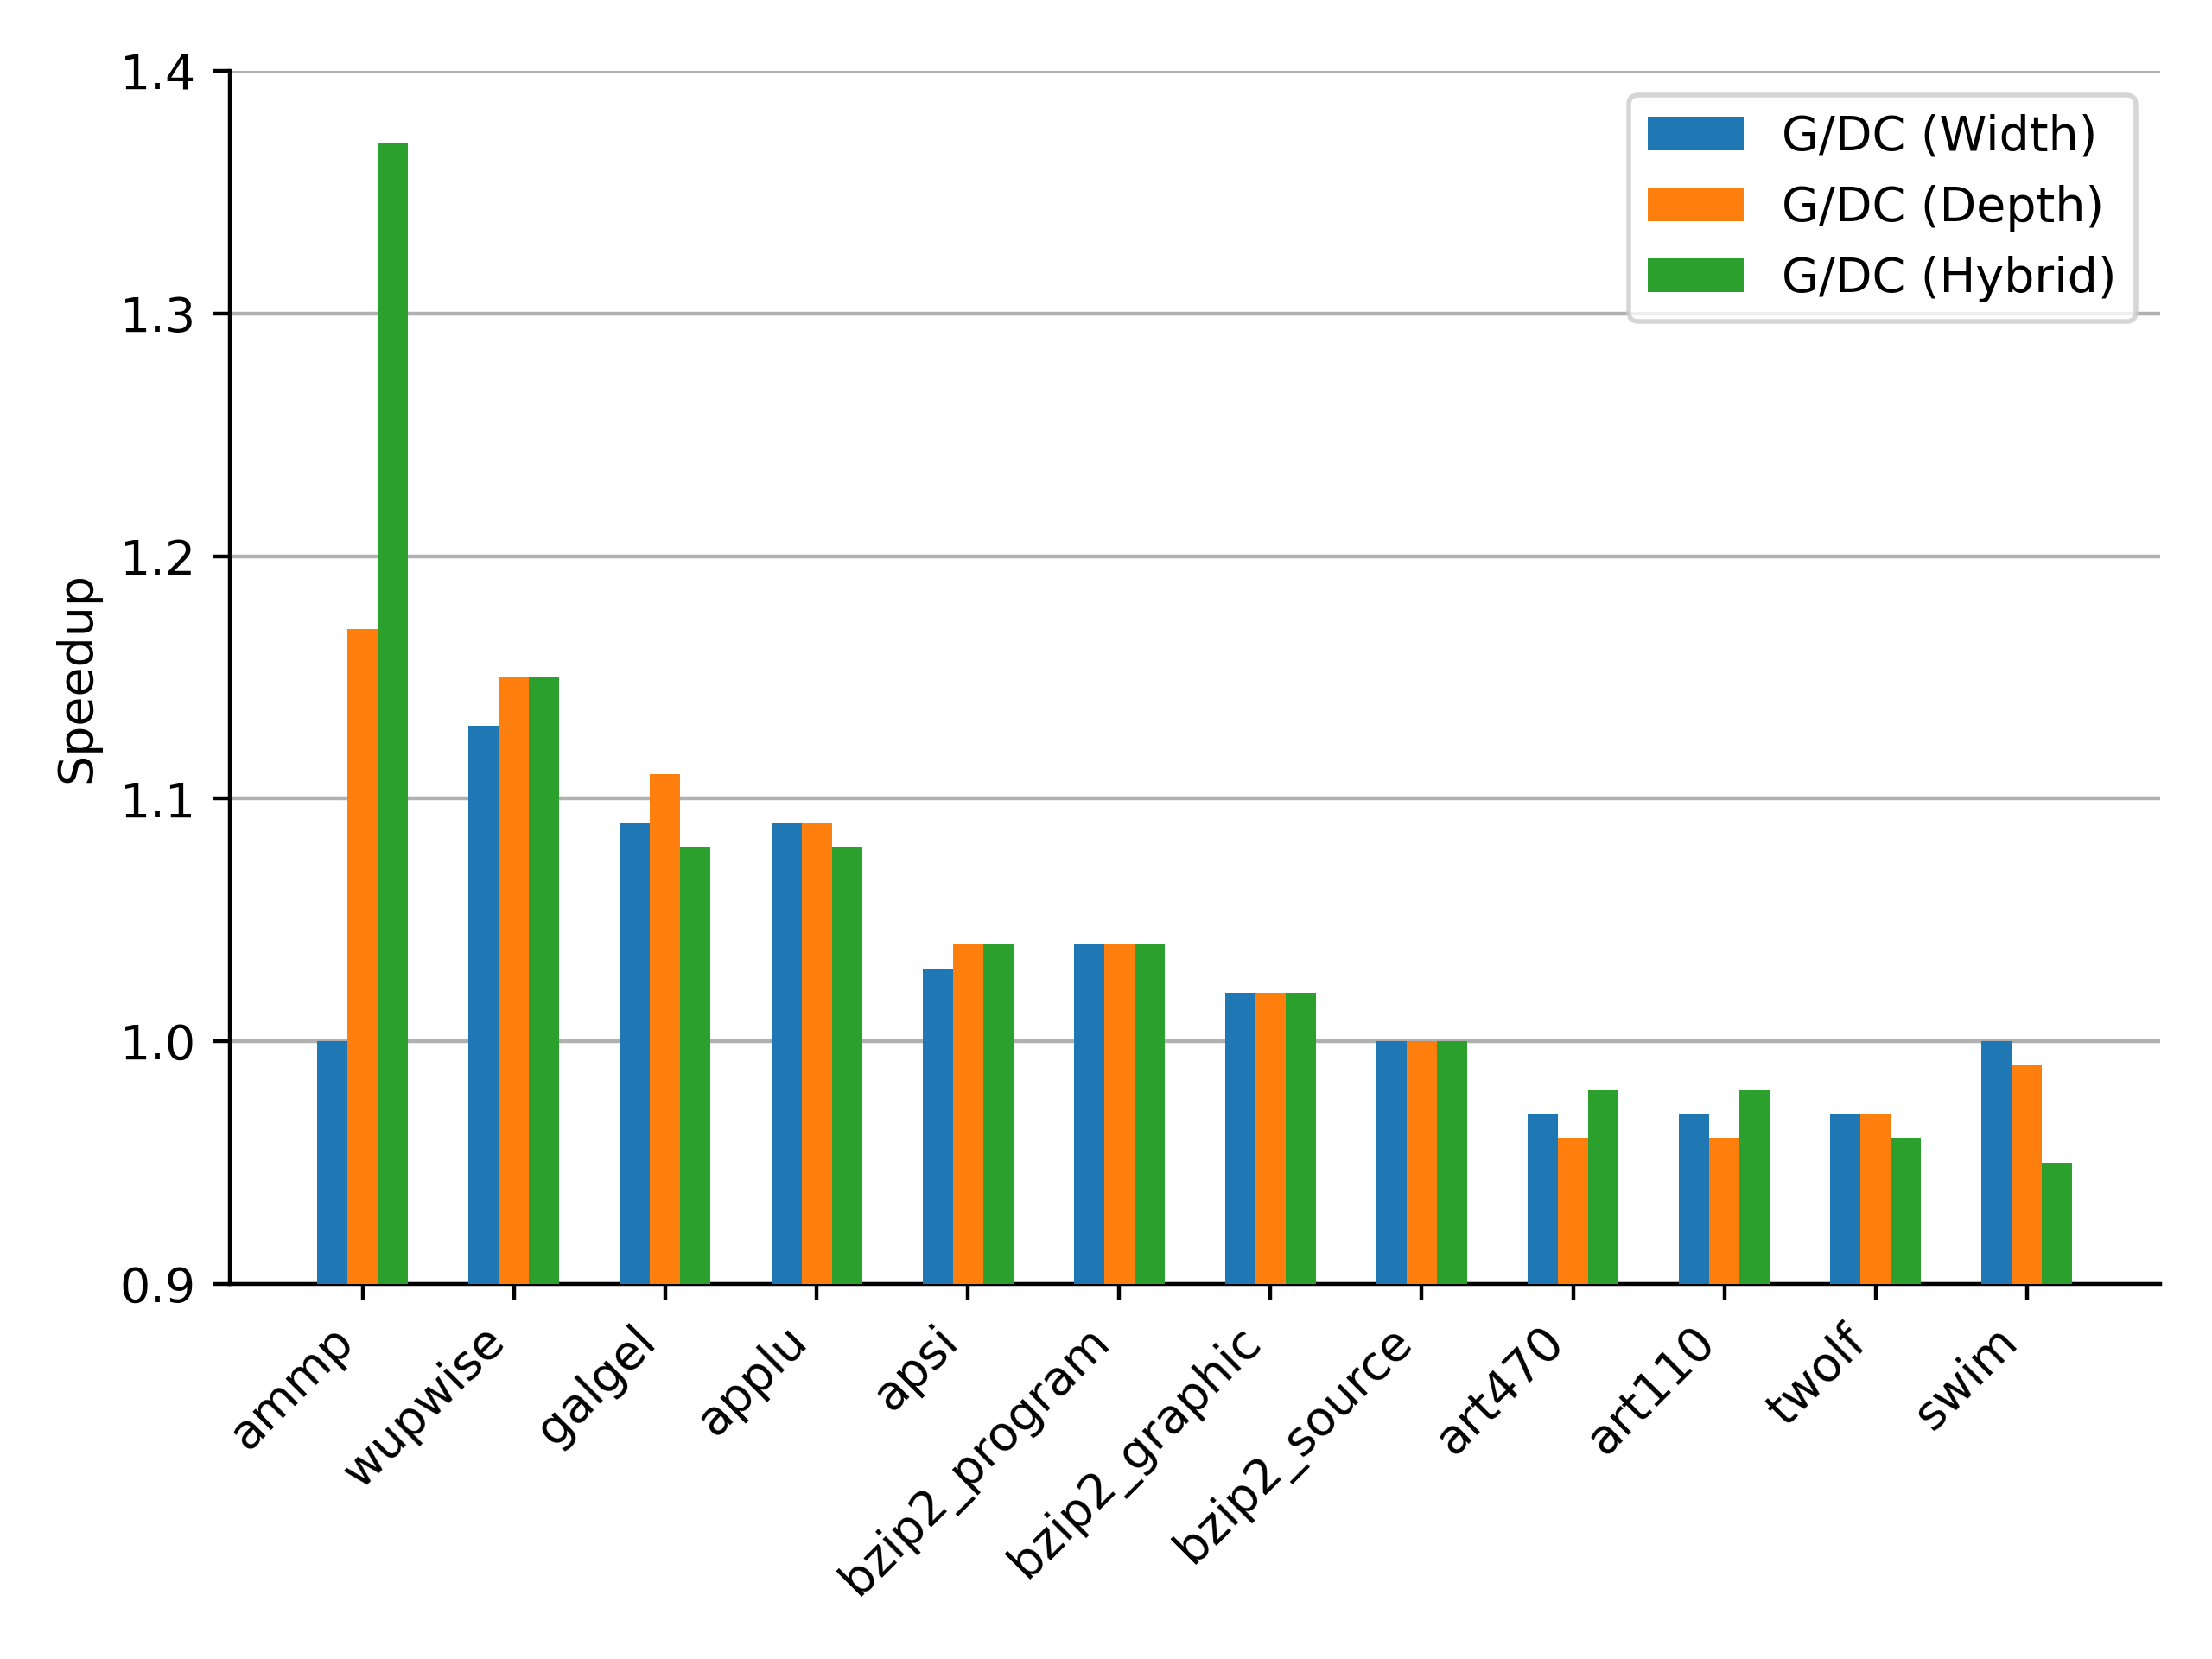
\includegraphics[width=90mm]{assets/tests.png}
    \vspace{-7mm}
    \caption{Speedup for the different benchmark tests.}
    \label{fig:tests}
\end{figure}

\subsection{Parameters}

The average speedup when varying the prefetch degree is presented in \cref{fig:speedup}. Prefetch degrees one and two yield a decent speedup. It seems prefetch degree four is the most optimal for all three variants. Increasing the prefetch degree further has a negative impact on the speedup. This decrease in speedup is likely caused by several factors. First, the higher the prefetcher degree, the more data is prefetched. A result of this is that less relevant data is prefetched, and useful cache lines may be evicted. This wastes processor cycles and pollutes the cache. Second, when there is not enough data in the GHB, the G/DC prefetcher becomes sequential. This is an inferior prefetcher scheme that does not yield a substantial speedup. Our findings show there is a clear trade-off between prefetching too much data, and not prefetching enough. The optimal prefetch degree in our implementation has been found to be four. 

\begin{figure}[H]
    \centering
    \vspace{-3mm}
     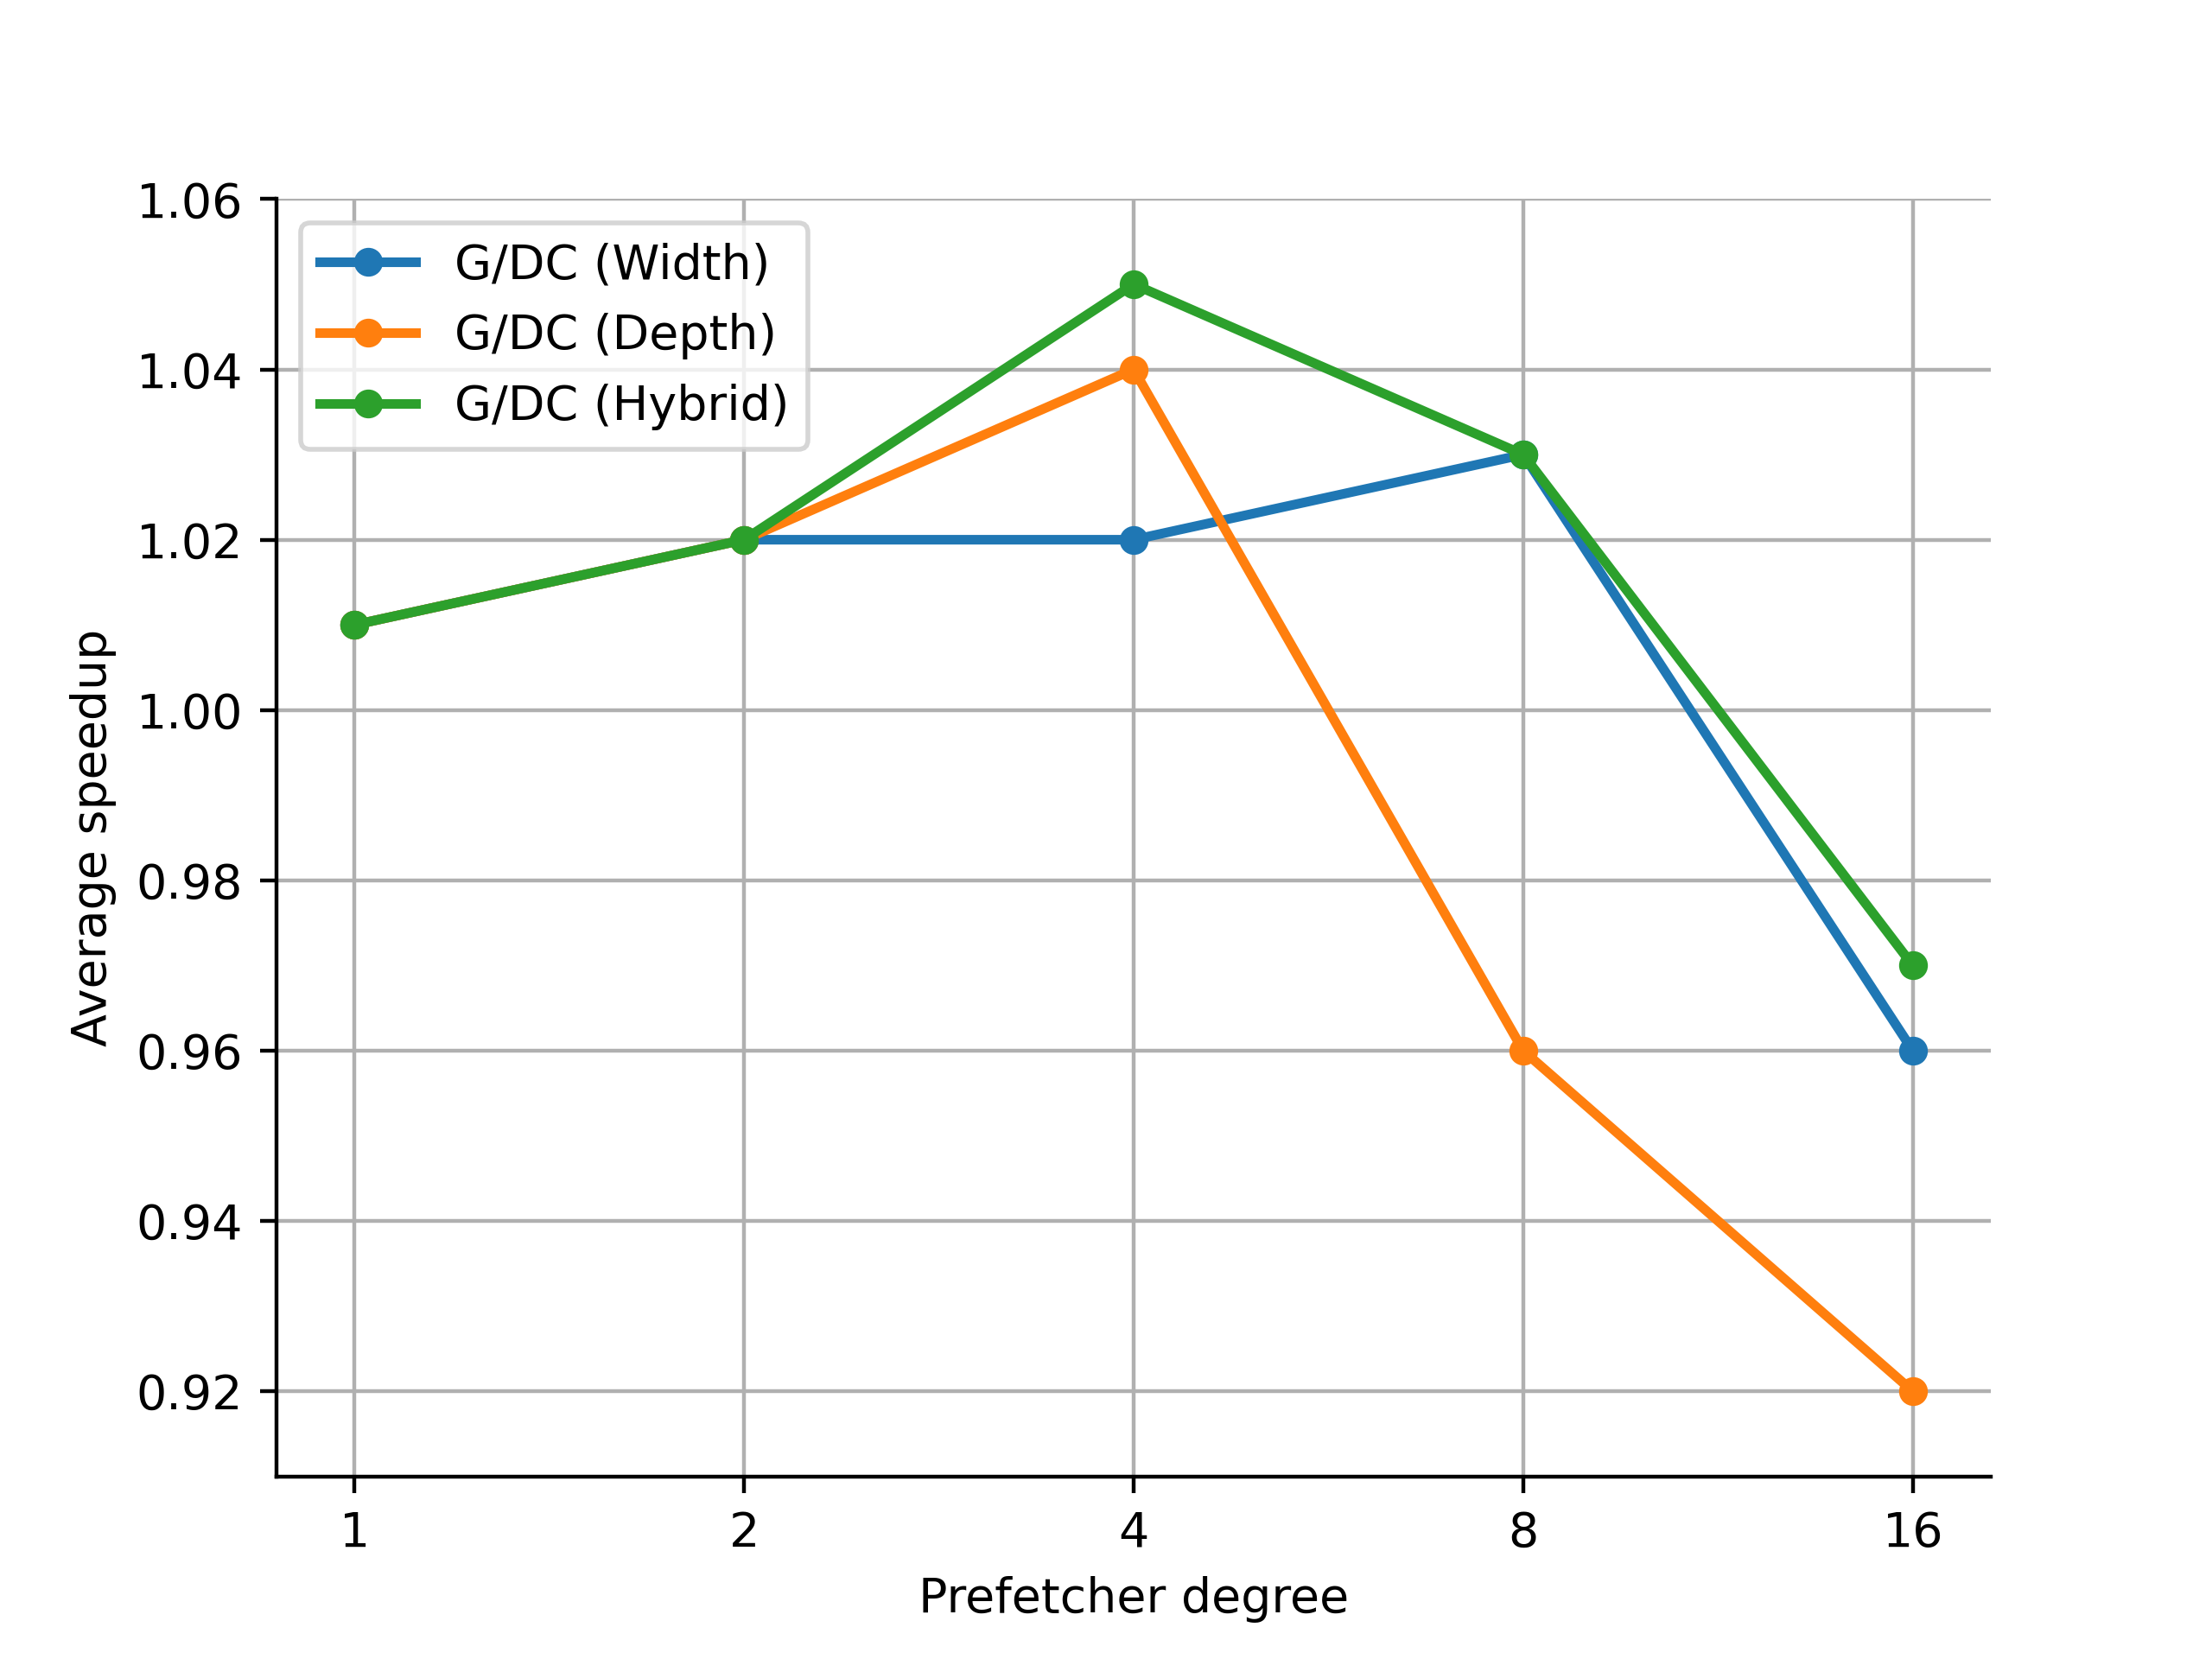
\includegraphics[width=90mm]{assets/speedup.png}
    \vspace{-7mm}
    \caption{Average speedup for different prefetch degrees.}
    \label{fig:speedup}
    \vspace{3mm}
\end{figure}

The average speedup achieved with different GHB and IT sizes is shown in \cref{fig:size}. The graph clearly shows that sizes smaller than 16 does not yield substantial speedups. It seems the minimum size for the GHB and IT is 16, and that going above this yields little performance gains. The highest speedup was achieved with size 256. These results are different from Nesbit and Smith's \cite{b1}. Their findings was that the ideal size was 512. However, our tests have been conducted with prefetch degree four, which may have impacted the results. Nesbit and Smith do not state how they found out 512 was the ideal size, but one can speculate this was found with a higher prefetching degree. The reason for this is that they found that the higher the prefetcher degree, the higher the speedup. We did not find that, and therefore our tests have been conducted with prefetch degree four. 

\begin{figure}[H]
    \centering
    \vspace{-3mm}
     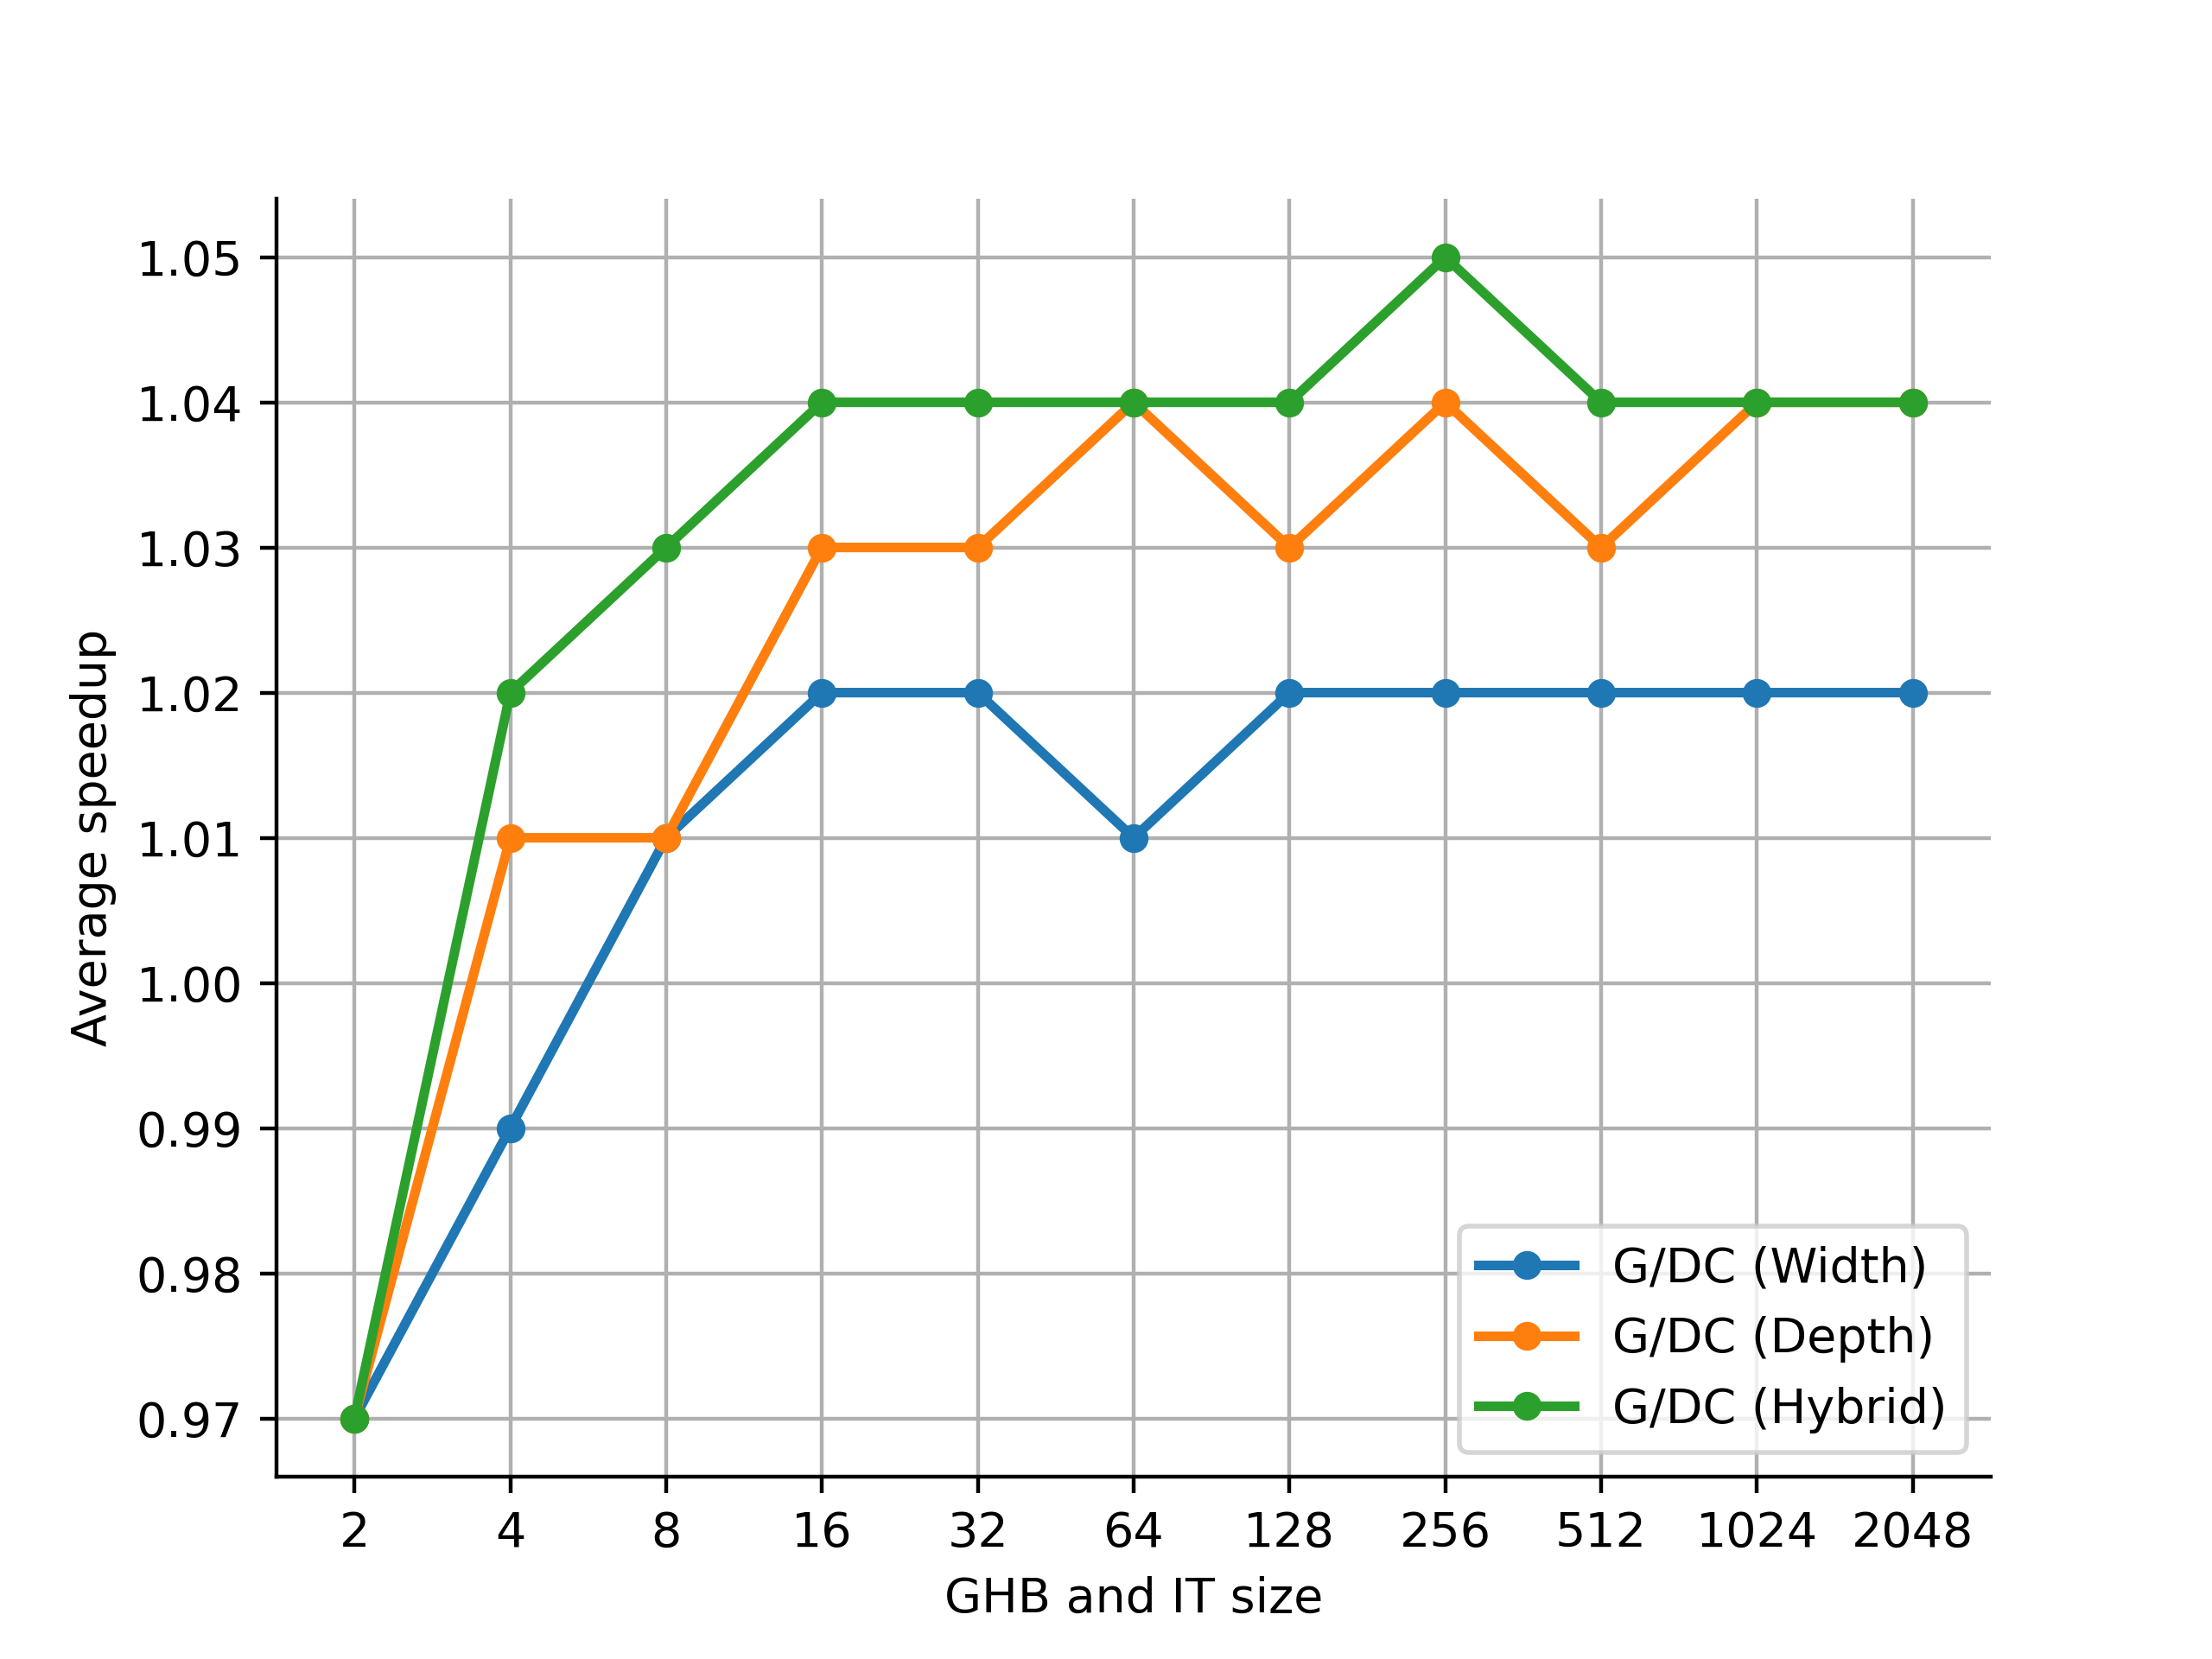
\includegraphics[width=90mm]{assets/size.png}
    \vspace{-7mm}
    \caption{Average speedup for different GHB and IT sizes.}
    \label{fig:size}
    \vspace{3mm}
\end{figure}

% ------------
% DISCUSSION
% ------------

\section{DISCUSSION}
\iffalse
This section might elaborate on alternative approaches that you have tried, but were not successful. It discusses weaknesses of your scheme and highlights the strong and weak points of your experimental setup.
\fi 

The best speedup was achieved with a GHB and IT size of 256. Going by Nesbit and Smith's calculations, this would require 4KB of storage \cite{b1}. In addition, a 2014 paper states that the size of the GHB and IT cause little hardware overhead \cite{falsafi}. Also, the prefetcher has been shown to achieve a speedup of 4\% with an IT and GHB size of 16. This means our prefetcher implementation should be realistic to implement in a processor without any substantial hardware overhead. 

A weakness with our test is the fact that we assumed the optimal GHB to IT ratio is 1:1. This is the ratio that Nesbit and Smith found to give the best performance \cite{b1}. However, our implementation runs on different hardware, so that ratio may not be optimal in our setup. Considering we were unable to achieve the same speedup as Nesbit and Smith, it could be fair to assume that our prefetcher could benefit from a different configuration. This could either improve the performance or enable us to achieve the same performance with even less silicone overhead.

Another weakness with our method is that we could have experimented more with the sequential fallback prefetcher. When there is no relevant data in the GHB, the prefetcher becomes sequential, and proceeds by prefetching enough data to satisfy the prefetch degree. We tested with and without the sequential fallback prefetcher, but found that generally the implementation benefited from it. We could have tweaked it, and for instance only used the sequential fallback prefetching when the MSHR queue was empty, or when it was not full. This would ensure the prefetcher would not prefetch too much data, even at higher prefetching degrees. 

% ------------
% RELATED WORK 
% ------------

\section{RELATED WORK}
\iffalse
The related work section puts your paper into a research context. It mentions other research with similar goals or schemes and compares them to your work, highlighting the commonalities and differences. It also shows whether you have an overview of the research area.
\fi 

    There are many other delta-correlation based prefetchers that aim to solve the same problem as G/DC. These all have different complexity costs and performance, and hence serve different purposes.

\subsection{PC/CD}
Also proposed by Nesbit and Smith \cite{b1}, PC/DC is a delta-correlation prefetcher. It uses delta pairs as correlation key by searching the delta stream in reverse order. This allows it to take better advantage of the GHB, hence lowering the size requirement for a given speedup.
They found that PC/DC was able to to achieve a slightly better performance while only occupying half the silicone real overhead of G/DC.

\subsection{DCPT}
Jahre et al. \cite{dcpt} proposed combining the table based design of RPT and delta-correlating design of PC/DC. This was done by using an RPT table in combination with a GHB and IT. The prefetcher used 4KB of silicone and was able to achieve a 27.2\% speedup over PC/DC, which is considered significant increase.

\subsection{Runahead Metadata}
Runahead MetaData (RMD) \cite{b6} is a pairwise-correlating data prefetcher. RMD uses two runahead metadata tables to predict what addresses/deltas might occur. This prefetcher has a small overhead, which is motivated by the movement towards multi-core processors where prefetchers needs to be simple and as low-overhead as possible \cite{b13}. RMD is considered state-of-the-art when it comes to pairwise-correlating data prefetchers \cite{b6}.

% ------------
% CONCLUSION 
% ------------

\section{CONCLUSION}
\iffalse
This section concludes your work by briefly repeating the goal of your work and stating the main results. It can also include planned future work. 
\fi 

This paper shows that Global Delta Correlation (G/DC) is a viable option for improving cache utilization. It has been tested and evaluated using the SPEC CPU2000 benchmark suite, and has been found to achieve an average speedup of 5\%. On single tests it has been able to achieve speedups of up to 37\%. This is on-par with many of the other prefetcher schemes it has been evaluated against. However, it seems G/DC is not able to recognize strided access patterns efficiently, as evident by the fact that it is outperformed by both DCPT-P and RPT. That being said, the G/DC prefetcher provides a reasonable speedup with little hardware overhead. 

% ------------
% BIBLIOGRAPHY 
% ------------

\bibliographystyle{IEEEtran}
\bibliography{references.bib}
\end{document}
